\chapter{Previous work - Rastermap Vectorization}
Image segmention has come a long way on images of normal everyday objects with deep CNNs. However none of the reviewed papers use their networks on raster maps. Not a lot of work has been done in regards to vectorization of raster maps using neural networks. However there has been a fair amount of research done on other techniques.

More work on satellite images.

Non artificial methods 

\section{Non-artifical intelligence methods}

\citeauthor{Leyk2010} presents a color image segmentation of raster maps from the \nth{19} century using the local image plane, frequency domain an color space. The goal of the color image segmentation is to reduce the color values to fit the original colors used when printing the map. 

In \cite{Iosifescu2016}, open-source solutions are used to vectorize historical maps from the \nth{19} century. Their procedure consist of five steps: Scanning of the map, georeferencing the map, pre-processing of image to clean artifacts, automatic vectorization, automaic cleaning of the results. The authors note that the pre-processing step and scan quality are the most crucial for the perfomance of the vectorization and has to be customized for each set of raster maps. The pre-processing consist of RGB channel processing, conversion to binary images and cleaning. By processing the RGB channels in the image, different features on the map can be highlighted. An example for the building extraction can be seen in \autoref{fig:map-preprocessing}. 

The pre-processed image is then converted to vector with Geospatial Data Abstraction Library\cite{OSGeo}(GDAL)'s polygonize and contour methods. The results are acceptable when taking the quality of the maps in to consideration.

\begin{figure}[H]
	\centering
	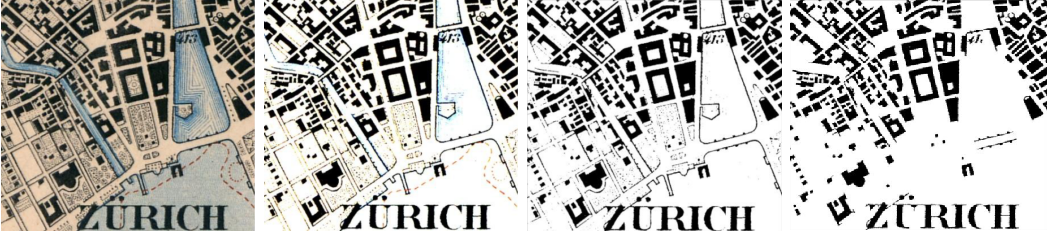
\includegraphics[width=\linewidth]{fig/map-processing.png}
	\captionsource{From left to right: Original image, RBG processed, binary representation and cleaned}{\citeauthor{Iosifescu2016}\cite{Iosifescu2016}}
	\label{fig:map-preprocessing}
\end{figure}


\subsection{Multi stage system}
\cite{Oka2012}


\section{Artificial intelligence methods}

\subsection{VecNET}
(Maybe not even relevant because of bad quality of paper and use of ANN?)

VecNet proposed by \citeauthor{Karabork2008} in 2008 is one of few examples of vectorization of cartographic raster maps using a neural network. The authors present a three-step process consisting of thinning, line tracking with ANN and simplification. The main goal of the network is to find the critical points of objects, that is, to find breakage points of lines. They use an ANN with an input layer, a hidden layer and an output layer to classify. The training set is very small with only 16 samples. The output layer is a single vector with size 12, where the 8 first places represent an 8-way chain code of directions (the direction the line is following) and the last four represent a prediction of where the next pixel is going to be. It evaluates if the point is critical by checking if the last 8-way direction is different from the one currently calculated. If the point is critical, they store it.

The algorithm is tested on a single raster map only consisting of lines and does not perform better than a sparse pixel algorithm, but manages to get acceptable results according to the authors.

\subsection{Knowledge based system}
\cite{Lee2000}

\cite{Song2000}


